\begin{appendix}
	\chapter{Configuration files}
		\lstinputlisting[label=lst:rb, language=C++, caption=Part of the gitlab configuration file.]{others/gitlab-cut.rb}
		\lstinputlisting[label=lst:fstab, language=C++, caption=Fstab confiuration file. Mount points to \gls{EFS}.]{others/fstab.txt}
	\chapter{Project screen-shots}
		\begin{figure}[!htbp]
			\centering
			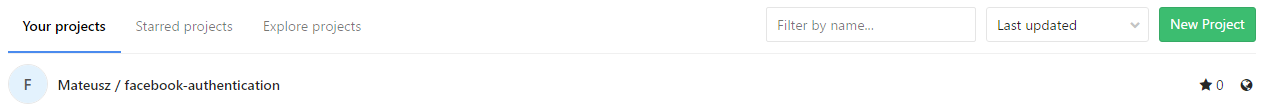
\includegraphics[width=1\textwidth]{img/ug-project/new-project2}
			\caption{Project list view.}
			\label{fig:project-list-view}
		\end{figure}		
		\begin{figure}[!htbp]
			\centering
			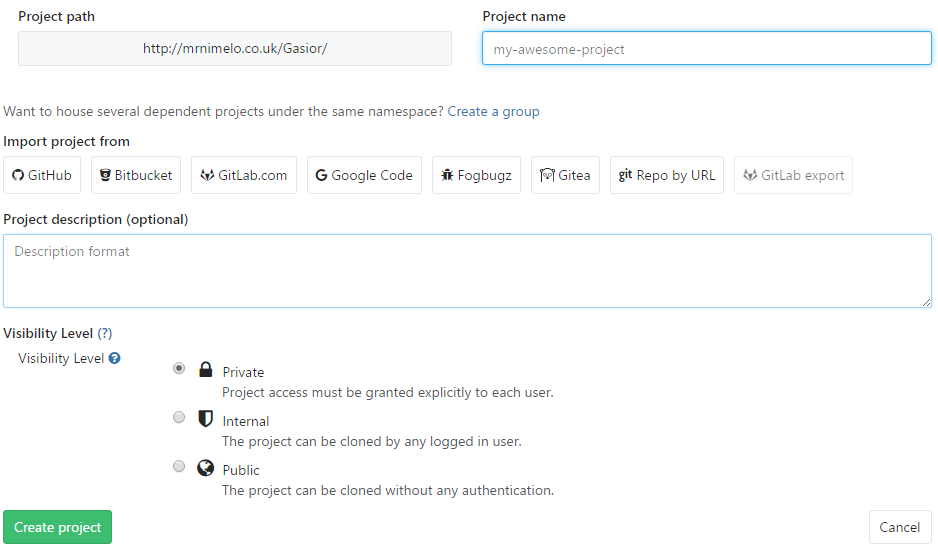
\includegraphics[width=1\textwidth]{img/ug-project/new-project-settings}
			\caption{New project settings panel.}
			\label{fig:project-settings}
		\end{figure}
		\begin{figure}[!htbp]
			\centering
			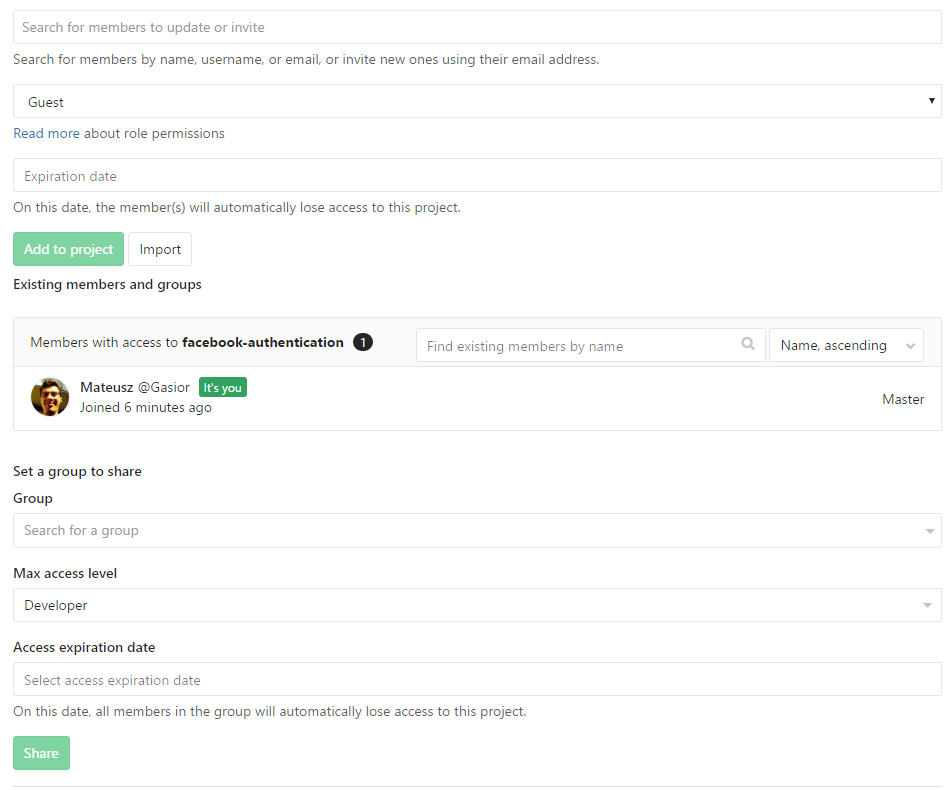
\includegraphics[width=1\textwidth]{img/ug-project/project-members-permissions}
			\caption{Project permissions panel.}
			\label{fig:project-members-permissions}
		\end{figure}
		\begin{figure}[!htbp]
			\centering
			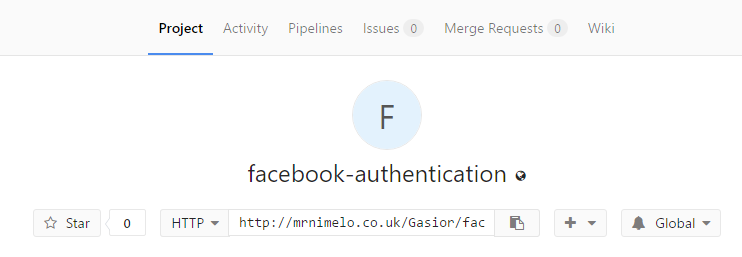
\includegraphics[width=1\textwidth]{img/ug-project/project-view}
			\caption{Project view panel.}
			\label{fig:project-view-panel}
		\end{figure}
		\begin{figure}[!htbp]
			\centering
			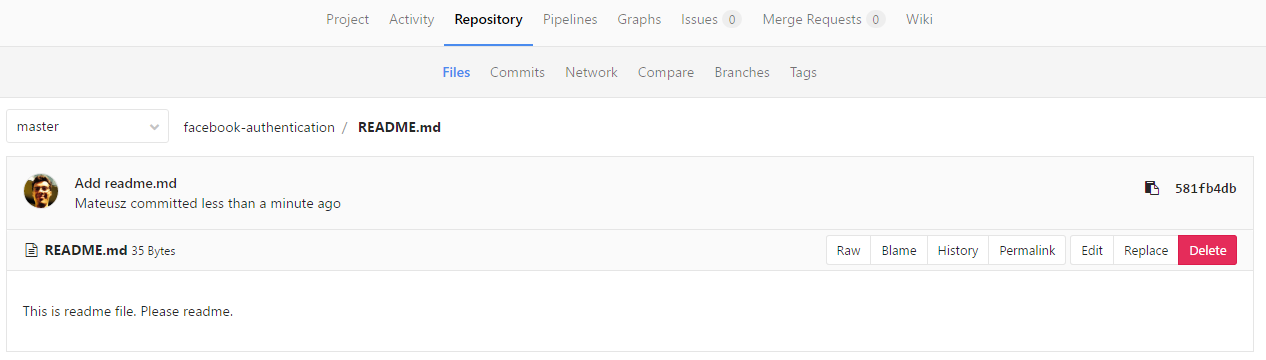
\includegraphics[width=1\textwidth]{img/ug-project/project-view2}
			\caption{Project repository view.}
			\label{fig:project-repository}
		\end{figure}
		\begin{figure}[!htbp]
			\centering
			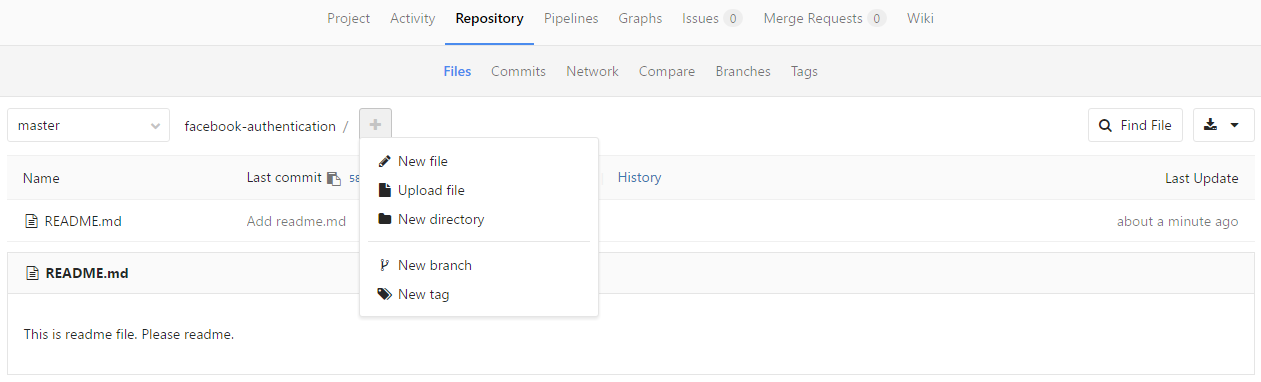
\includegraphics[width=1\textwidth]{img/ug-project/project-view-repository}
			\caption{Project members view panel.}
			\label{fig:project-members}
		\end{figure}
	\chapter{Group screen-shots}
		\begin{figure}[!htbp]
			\centering
			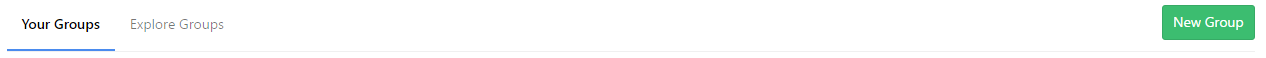
\includegraphics[width=1\textwidth]{img/ug-groups/new-group1}
			\caption{Creating group view.}
			\label{fig:creating-group-view}
		\end{figure}	
		\begin{figure}[!htbp]
			\centering
			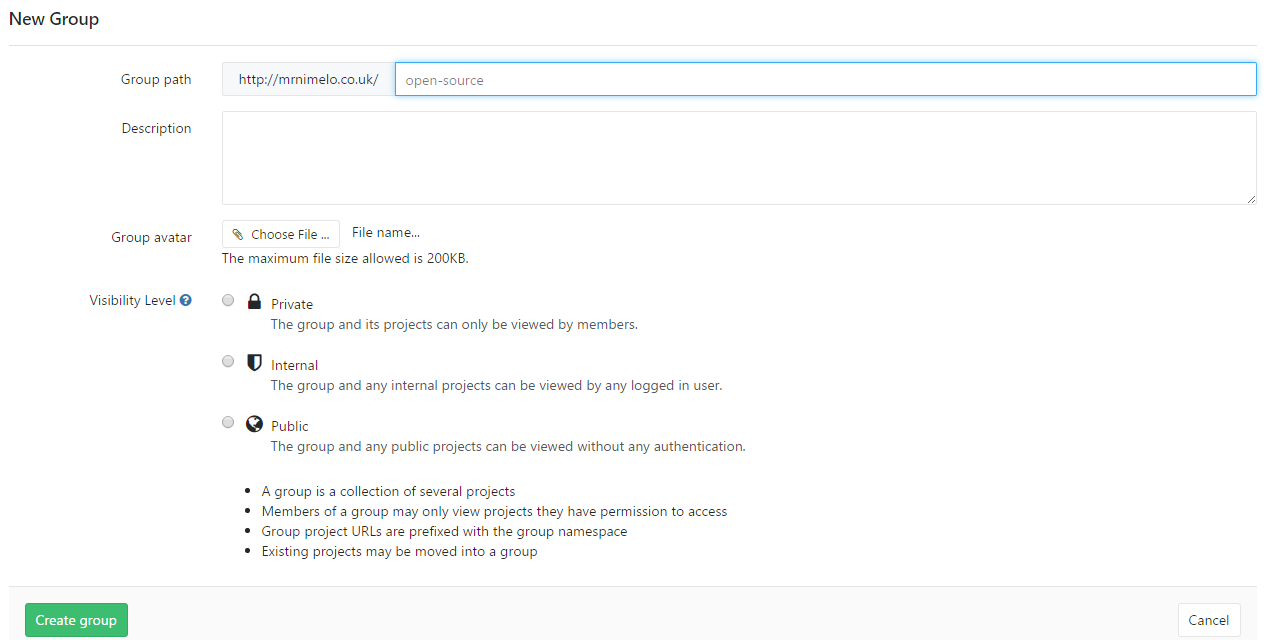
\includegraphics[width=1\textwidth]{img/ug-groups/new-group-settings}
			\caption{Group settings view.}
			\label{fig:group-settings-view}
		\end{figure}
		\begin{figure}[!htbp]
			\centering
			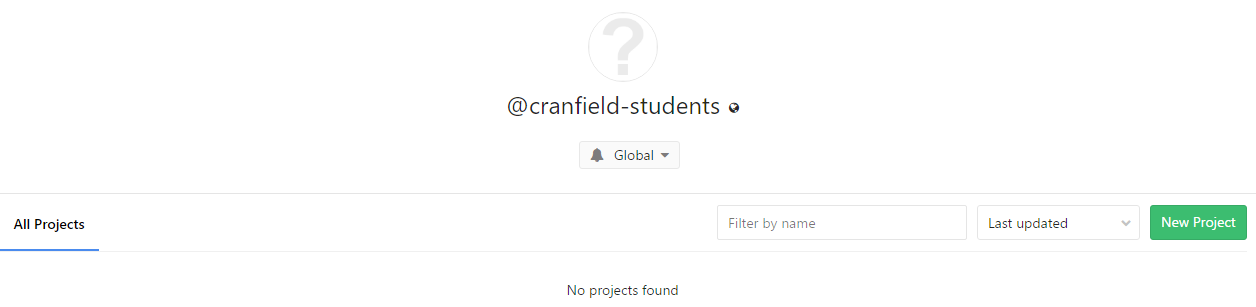
\includegraphics[width=1\textwidth]{img/ug-groups/group-projects}
			\caption{Adding project to group view.}
			\label{fig:adding-project-to-group}
		\end{figure}		
		\begin{figure}[!htbp]
			\centering
			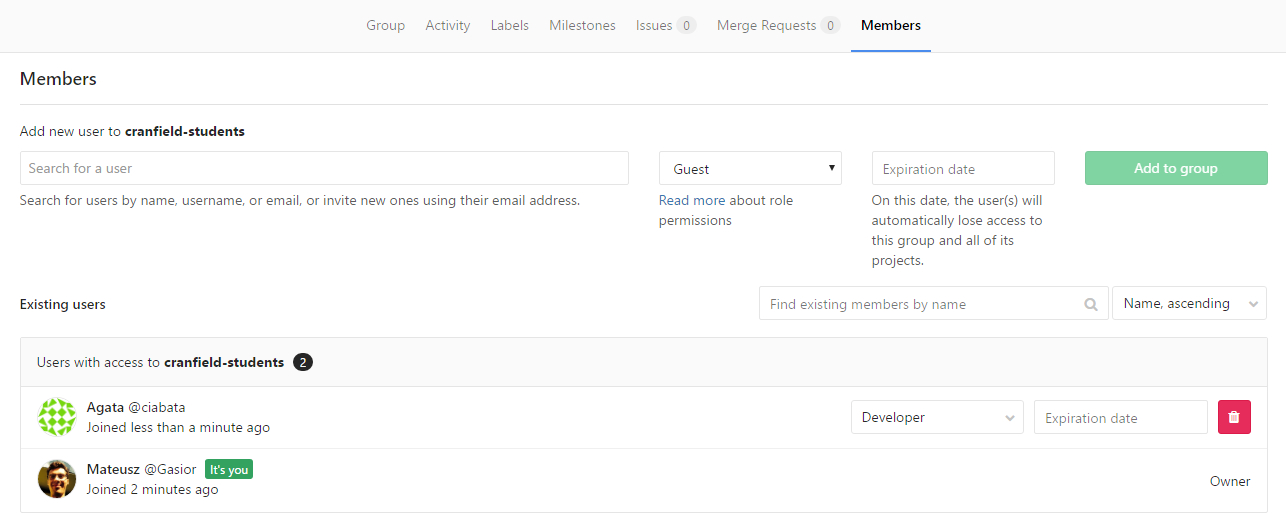
\includegraphics[width=1\textwidth]{img/ug-groups/group-members}
			\caption{Adding user to group view.}
			\label{fig:adding-user-to-group}
		\end{figure}		
	\chapter{Administration screen-shots}
		\begin{figure}[!htbp]
			\centering
			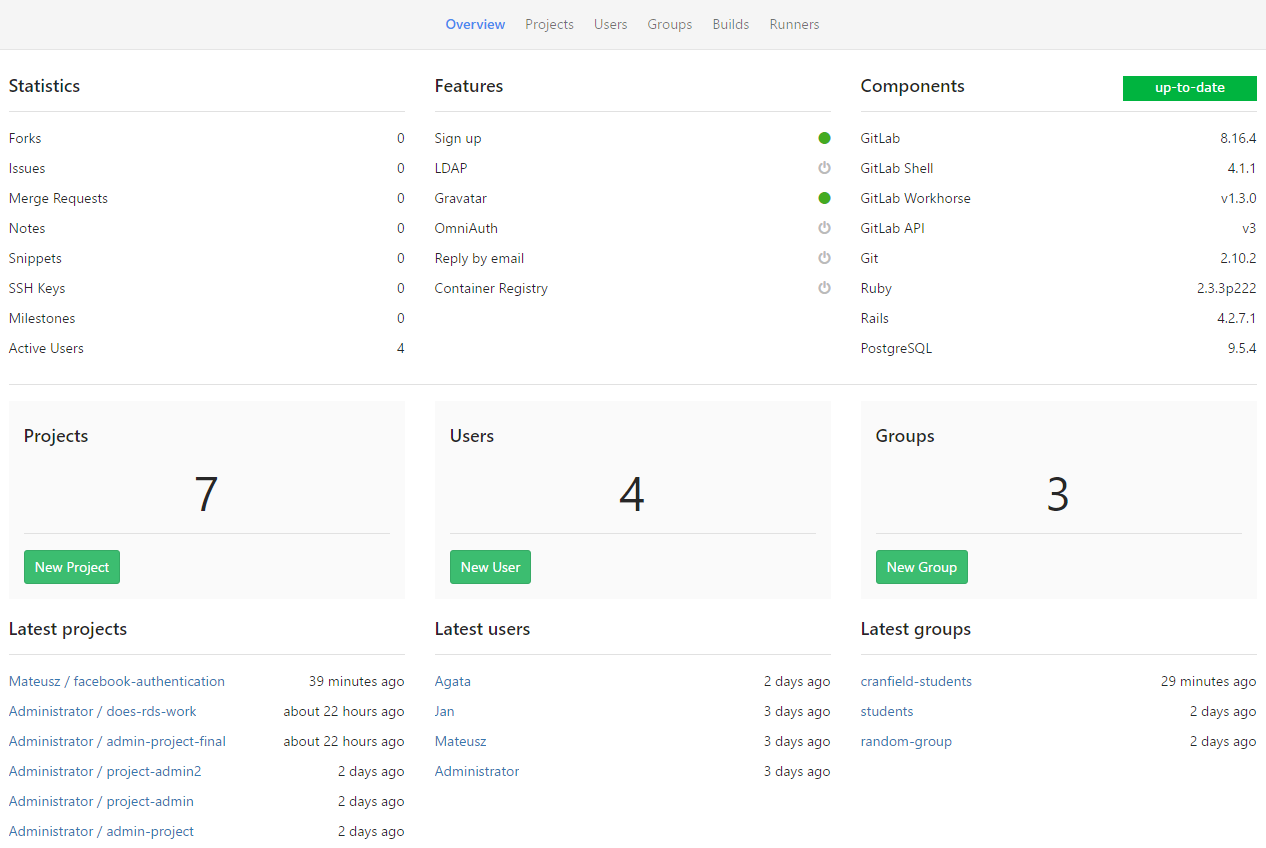
\includegraphics[width=1\textwidth]{img/ug-administartion/overview}
			\caption{Administration overview view.}
			\label{fig:administration-overview-view}
		\end{figure}		
		\begin{figure}[!htbp]
			\centering
			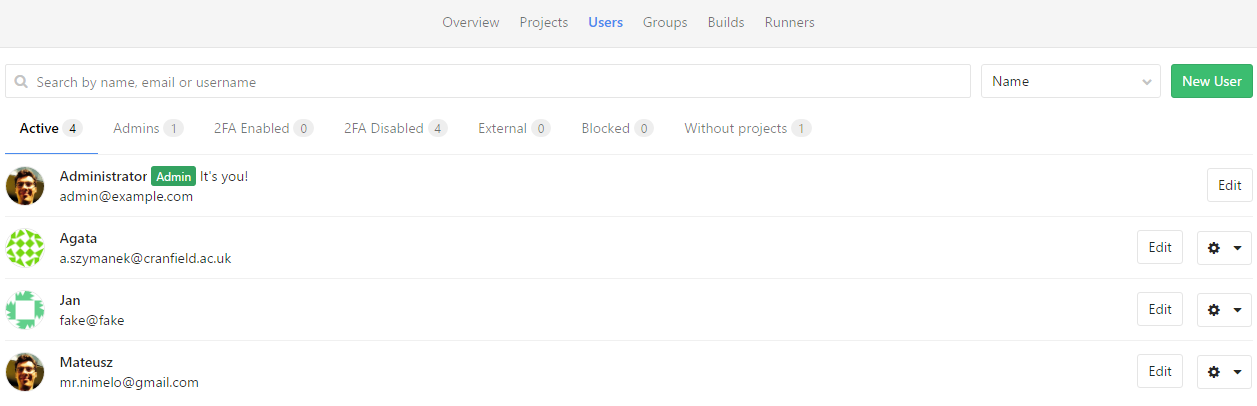
\includegraphics[width=1\textwidth]{img/ug-administartion/users}
			\caption{User administration view.}
			\label{fig:user-administration-view}
		\end{figure}
		\begin{figure}[!htbp]
			\centering
			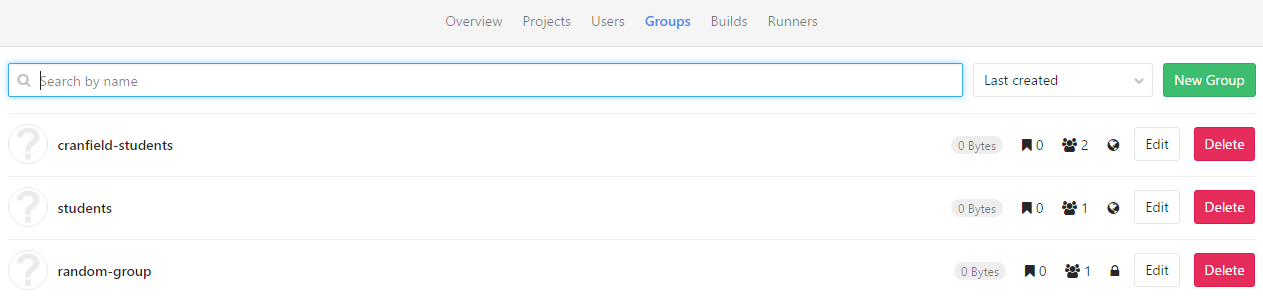
\includegraphics[width=1\textwidth]{img/ug-administartion/groups}
			\caption{Groups administration view.}
			\label{fig:groups-administration-view}
		\end{figure}		
		\begin{figure}[!htbp]
			\centering
			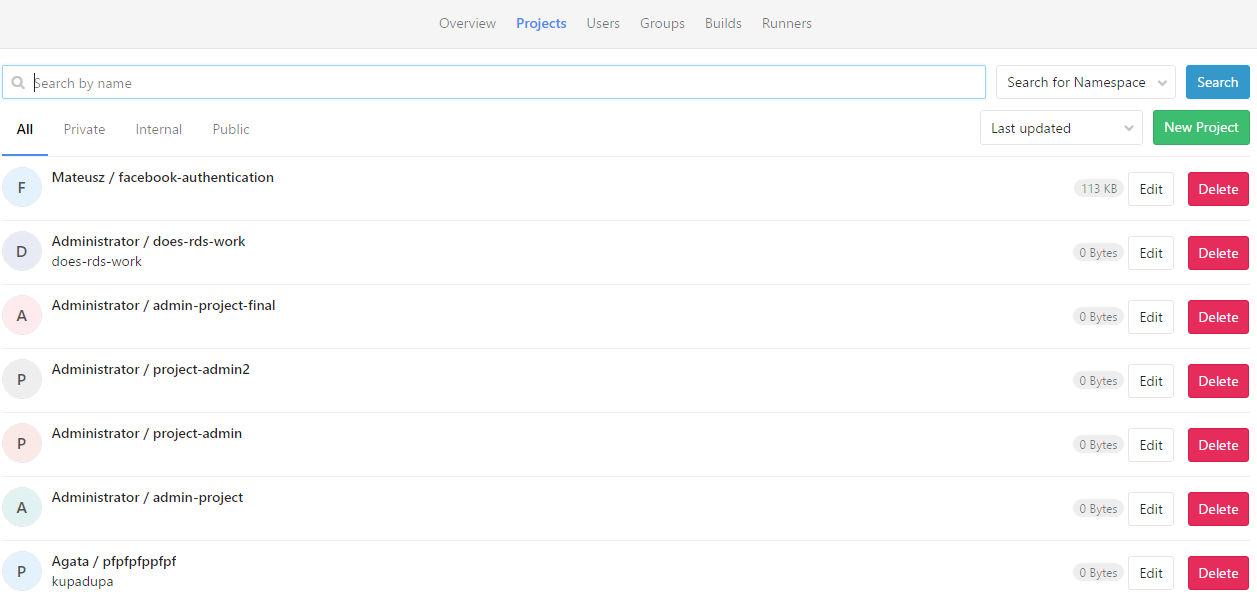
\includegraphics[width=1\textwidth]{img/ug-administartion/projects}
			\caption{Projects administration view.}
			\label{fig:projects-administration-view}
		\end{figure}		
		\begin{figure}[!htbp]
			\centering
			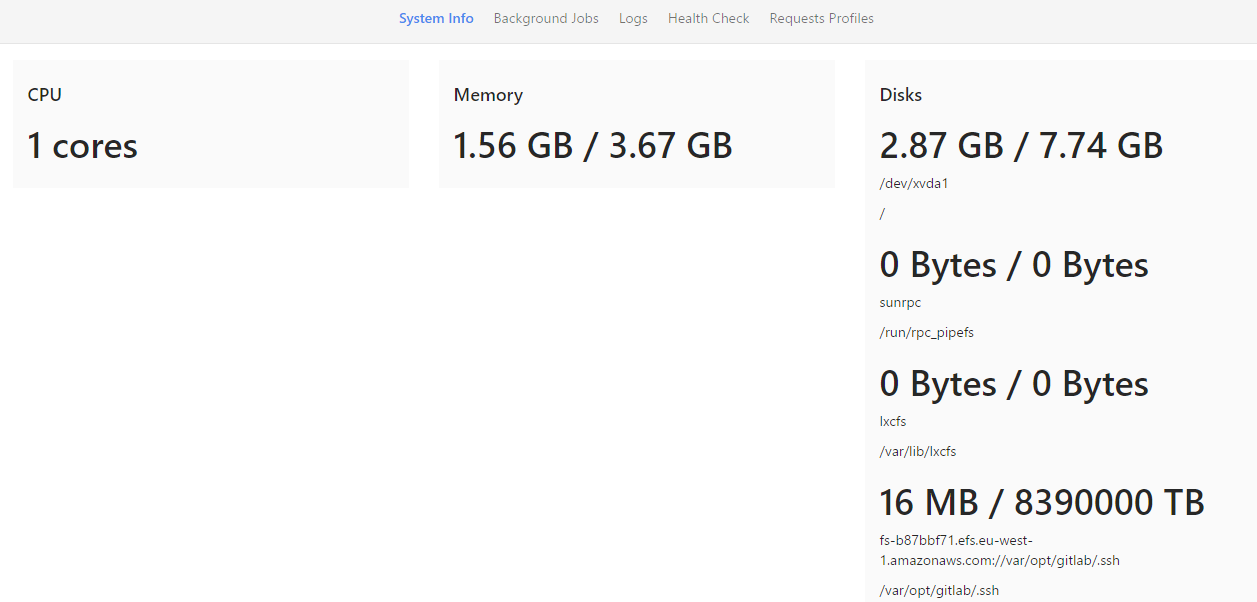
\includegraphics[width=1\textwidth]{img/ug-administartion/monitoring}
			\caption{Monitoring of resource usage view.}
			\label{fig:resource-usage-view}
		\end{figure}		
\end{appendix}